\section{Approach}
\label{sec:approach}
We propose a modular framework for representation learning and transfer learning. 
The framework consists three modules: 
\begin{enumerate}
	\item the representation learner, which constructs an abstract representation of the task environment
	\item the policy learner is RL learner which operates based on the task abstraction created by the representation learner. 
	\item the task environment. RL tasks to be solved by the RL learner
\end{enumerate}

History approach vs parallel approach.


\subsection{Representation Learners}
The representation learner aims to construct an abstract and generalized representation of the task environment to facilitate later knowledge transfer.
Our framework includes several architectures as visualized in Figure \ref{fig:repr_learner}.
The architectures all include some lower-dimensional ``bottleneck'' layers, 
which are designed to enforce dimensionality reduction of the input.
Once learned, this intermediate latent space is expected to create a more compact and abstract representation of the original environment and serve as the basis of transfer learning. 

\begin{figure}[ht!]
	\centering
	\begin{subfigure}{0.45\columnwidth}
		\centering
		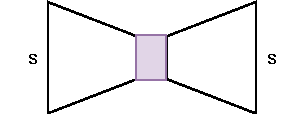
\includegraphics[width=\linewidth]{../img/very_simple_autoencoder.pdf}
		\caption{Simple autoencoder}
		\label{subfig:repr_learner_simple_autoencoder}
	\end{subfigure}%
	~ 
	\begin{subfigure}{0.45\columnwidth}
		\centering
		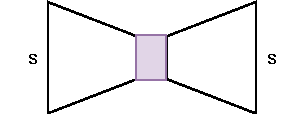
\includegraphics[width=\linewidth]{../img/very_simple_autoencoder.pdf}
		\caption{Variational autoencoder}
		\label{subfig:repr_learner_vae}
	\end{subfigure}
	\begin{subfigure}{0.5\columnwidth}
		\centering
		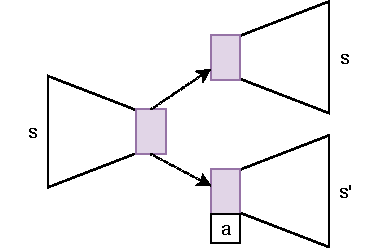
\includegraphics[width=\linewidth]{../img/janus.pdf}
		\caption{Janus}
		\label{subfig:repr_learner_janus}
	\end{subfigure}%
	~ 
	\begin{subfigure}{0.5\columnwidth}
		\centering
		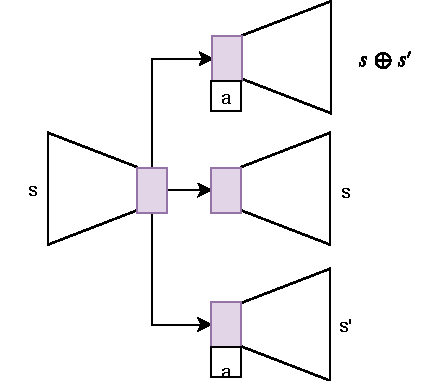
\includegraphics[width=\linewidth]{../img/cerberus.pdf}
		\caption{Cerberus}
		\label{subfig:repr_learner_cerberus}
	\end{subfigure}
	\caption{Network architectures of of representation learner, where $s$ and $s'$ indicate current and next state respectively, and $a$ indicates the action leading from $s$ to $s$. The layers marked in purple are the latent representations to be used as the basis of later transfer learning.}
	\label{fig:repr_learner}
\end{figure}


\subsubsection{Simple Autoencoder}
The simple autoencoder seeks to 
, as shown in Figure \ref{subfig:repr_learner_simple_autoencoder}.

\begin{itemize}
	\item simply reconstruction of input
\end{itemize}

\subsubsection{Variational Autoencoder}
, as shown in Figure \ref{subfig:repr_learner_vae}.

\begin{itemize}
	\item continuous
\end{itemize}

\subsubsection{Janus}
, as shown in Figure \ref{subfig:repr_learner_janus}.
\begin{itemize}
	\item preserve transition dynamics
\end{itemize}

\subsubsection{Cerberus}
, as shown in Figure \ref{subfig:repr_learner_cerberus}.

\begin{itemize}
	\item preserve transition dynamics
\end{itemize}

\subsection{Policy Learners}
Based on the latent space constructed by the representation learner (marked in purple), the policy learner is RL agent that...

learn values of states.

\subsubsection{Table-based(?)}

\subsubsection{DQN}
DQN \citep{DQN}, prioritized memory \citep{prioritized_memory}
\begin{itemize}
	\item bypass the exponential growth with state configurations
\end{itemize}

\subsubsection{DDQN}
DDQN \citep{DDQN}, Dueling DQN \citep{DuelingDQN}

\begin{itemize}
	\item target model
\end{itemize}